\chapter{Data Mass and Orbital Dynamics in Continuous Learning}

\begin{tcolorbox}[colback=DarkSkyBlue!5!white,colframe=DarkSkyBlue!75!black,title=Chapter Summary]
This chapter introduces the concept of data-induced mass perturbation in the Elder-Mentor-Erudite system and its crucial role in enabling autonomous continuous learning. We examine how newly acquired data produces temporal mass disturbances in Erudite entities, propagating orbital disruptions through the hierarchical system. These precisely quantified disruptions initiate adaptive rebalancing processes, effectively translating raw data inflows into knowledge integration across multiple scales. Through rigorous mathematical formulation, we demonstrate how this mechanism creates a self-regulating, perpetual learning system when operated in an indefinite loop, establishing the theoretical foundations for truly autonomous knowledge acquisition without human intervention.
\end{tcolorbox}

\section{Introduction to Data-Mass Coupling}

The fundamental connection between data acquisition and entity mass in the Elder Heliosystem represents one of the most significant mechanisms for autonomous continuous learning. Unlike static learning systems that require explicit optimization schedules, the Elder Heliosystem exhibits intrinsic adaptation through the orbital dynamics of its constituent entities when subjected to data-induced mass fluctuations.

\begin{definition}[Data-Mass Coupling]
Data-Mass Coupling is the mechanism by which newly introduced data temporarily modifies the effective mass of an Erudite entity, expressed as:
\begin{equation}
m_{\text{Erudite}}(t) = m_{\text{base}} + \Delta m_{\text{data}}(t)
\end{equation}
where $\Delta m_{\text{data}}(t)$ is the temporal mass perturbation induced by data acquisition at time $t$.
\end{definition}

This seemingly simple mechanism initiates a cascade of orbital adjustments that propagate upward through the hierarchical structure, enabling the entire system to adapt continuously to new information without external supervision.

\section{Temporal Dynamics of Data-Induced Mass Fluctuations}

When an Erudite entity encounters new data, it experiences a temporary increase in effective mass proportional to the information content and novelty of the data. This mass increase is not permanent but follows a characteristic decay pattern as the knowledge is integrated.

\begin{proposition}[Data-Mass Temporal Dynamics]
The temporal evolution of data-induced mass follows:
\begin{equation}
\Delta m_{\text{data}}(t) = \sum_{i} I(D_i) \cdot N(D_i, \theta_{\text{Erudite}}) \cdot e^{-\lambda_i(t-t_i)}
\end{equation}
where:
\begin{itemize}
    \item $I(D_i)$ is the information content of data point $D_i$
    \item $N(D_i, \theta_{\text{Erudite}})$ is the novelty factor relative to current parameters
    \item $\lambda_i$ is the knowledge integration rate
    \item $t_i$ is the time when data point $D_i$ was introduced
\end{itemize}
\end{proposition}

The novelty factor $N(D_i, \theta_{\text{Erudite}})$ plays a crucial role, as it ensures that only data containing information not already encoded in the Erudite's parameters will generate significant mass perturbations. This natural filtering mechanism prevents redundant learning.

\section{Orbital Disruption Propagation}

\subsection{Primary Effects on Erudite Orbits}

The temporary mass increase of an Erudite entity disrupts its orbital trajectory around its parent Mentor. According to Elder orbital mechanics, this mass increase has precisely quantifiable effects on orbital parameters.

\begin{theorem}[Erudite Orbital Disruption]
A temporal mass increase $\Delta m_{\text{data}}$ in an Erudite entity modifies its orbital parameters as follows:
\begin{align}
r_{\text{new}} &= r_{\text{old}} \cdot \left(1 - \frac{\Delta m_{\text{data}}}{m_{\text{base}} + \Delta m_{\text{data}}}\right) \\
\omega_{\text{new}} &= \omega_{\text{old}} \cdot \sqrt{\frac{m_{\text{base}}}{m_{\text{base}} + \Delta m_{\text{data}}}}
\end{align}
where $r$ is the orbital radius and $\omega$ is the angular velocity.
\end{theorem}

\begin{proof}
From the Elder gravitational law, we know that the orbital radius is inversely proportional to the mass of the orbiting entity when the central mass remains constant. The conservation of angular momentum requires that $r^2\omega$ remains constant, leading to the derived relationships.
\end{proof}

Figure \ref{fig:erudite_orbit_perturbation} illustrates this orbital disruption process.

\begin{figure}[ht]
\centering
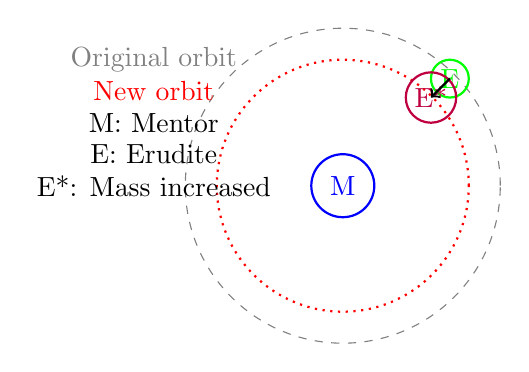
\begin{tikzpicture}[scale=0.8]
    % Mentor at center - simple circle
    \draw[thick, blue] (0,0) circle (0.5cm);
    \node[blue] at (0,0) {M};
    
    % Original orbit
    \draw[dashed, gray] (0,0) circle (2.5cm);
    
    % New orbit  
    \draw[dotted, thick, red] (0,0) circle (2cm);
    
    % Erudite positions - simple circles
    \draw[thick, green] (1.7,1.7) circle (0.3cm);
    \node[green] at (1.7,1.7) {E};
    
    \draw[thick, purple] (1.4,1.4) circle (0.4cm);
    \node[purple] at (1.4,1.4) {E*};
    
    % Simple arrow
    \draw[->, thick] (1.7,1.7) -- (1.4,1.4);
    
    % Labels
    \node[gray] at (-3,2) {Original orbit};
    \node[red] at (-3,1.5) {New orbit};
    \node at (-3,1) {M: Mentor};
    \node at (-3,0.5) {E: Erudite};
    \node at (-3,0) {E*: Mass increased};
    
\end{tikzpicture}
\caption{Orbital perturbation of an Erudite entity due to data-induced mass increase.}
\label{fig:erudite_orbit_perturbation}
\end{figure}

\subsection{Secondary Effects on Mentor Entities}

The orbital disruptions at the Erudite level propagate upward to affect the Mentor entities through gravitational coupling. This represents the bottom-up knowledge transfer mechanism in the Elder framework.

\begin{proposition}[Mentor Response to Erudite Disruption]
The orbital parameters of a Mentor entity respond to Erudite disruptions according to:
\begin{equation}
\Delta \vec{v}_{\text{Mentor}} = \sum_{j \in \text{Erudites}} G \frac{m_j \Delta m_j}{|\vec{r}_{\text{Mentor}} - \vec{r}_j|^2} \hat{r}_{j \to \text{Mentor}}
\end{equation}
where $G$ is the Elder gravitational constant, $m_j$ is the mass of Erudite $j$, and $\hat{r}_{j \to \text{Mentor}}$ is the unit vector from Erudite $j$ to the Mentor.
\end{proposition}

This velocity perturbation causes the Mentor to adjust its own orbit around the Elder, albeit with a dampened effect due to the Mentor's greater mass. This dampening ensures that only significant or consistent Erudite disruptions influence higher-level knowledge structures.

\subsection{Tertiary Effects on the Elder Entity}

Finally, the orbital adjustments of multiple Mentors introduce minute perturbations to the Elder entity itself, representing the slowest but most profound learning mechanism in the system.

\begin{theorem}[Elder Adaptation Rate]
The adaptation rate of Elder parameters in response to data-induced disruptions follows:
\begin{equation}
\frac{d\theta_{\text{Elder}}}{dt} \propto \sum_{k \in \text{Mentors}} \alpha_k \sum_{j \in \text{Erudites}_k} \beta_j \Delta m_{\text{data},j}
\end{equation}
where $\alpha_k$ and $\beta_j$ are coupling coefficients determining the strength of influence from each hierarchical level.
\end{theorem}

This multi-level propagation mechanism creates a natural learning hierarchy where:
\begin{itemize}
    \item Erudite entities adapt rapidly to new data (seconds to minutes in computational time)
    \item Mentor entities evolve more gradually, integrating consistent patterns (minutes to hours)
    \item The Elder entity evolves very slowly, only incorporating universal principles (hours to days)
\end{itemize}

\section{Autonomous Learning Through Continuous Orbital Dynamics}

\subsection{The Perpetual Learning Cycle}

When operated in an indefinite loop, the Elder system achieves autonomous continuous learning without external intervention. Figure \ref{fig:perpetual_learning_cycle} illustrates this self-sustaining cycle.

\begin{figure}[h]
\centering
\begin{tikzpicture}[
    node distance=2cm,
    block/.style={rectangle, draw, rounded corners, minimum width=2.5cm, minimum height=1cm, align=center},
    arrow/.style={thick,->,>=stealth},
    scale=0.85
    ]
    
    % Process blocks
    \node[block, fill=yellow!20] (data) {New Data Ingestion};
    \node[block, fill=green!20, right=of data] (mass) {Erudite Mass Perturbation};
    \node[block, fill=blue!20, below=of mass] (orbit) {Orbital Disruption Cascade};
    \node[block, fill=red!20, below=of data] (learning) {Multi-level Parameter Updates};
    \node[block, fill=purple!20, left=of learning] (integration) {Knowledge Integration};
    
    % Arrows
    \draw[arrow] (data) -- (mass);
    \draw[arrow] (mass) -- (orbit);
    \draw[arrow] (orbit) -- (learning);
    \draw[arrow] (learning) -- (integration);
    \draw[arrow] (integration) to[bend right=30] node[left, align=center] {System stabilizes\\temporarily} (data);
    
    % Cycle
    \node[draw, dashed, rounded corners, fit=(data) (mass) (orbit) (learning) (integration), inner sep=0.5cm] {};
    \node[above] at (data.north) {Perpetual Learning Cycle};
    
\end{tikzpicture}
\caption{The perpetual learning cycle in the Elder system when operated with continuous data ingestion. The cycle maintains itself through orbital dynamics without requiring external optimization schedules.}
\label{fig:perpetual_learning_cycle}
\end{figure}

\subsection{Mathematical Formalism for Continuous Operation}

The autonomous learning capability can be formalized through a system of coupled differential equations:

\begin{align}
\frac{d\vec{r}_{\text{Erudite},j}}{dt} &= \vec{v}_{\text{Erudite},j} \\
\frac{d\vec{v}_{\text{Erudite},j}}{dt} &= \vec{a}_{\text{gravity},j} + \vec{a}_{\text{data-mass},j}(t) \\
\frac{d\theta_{\text{Erudite},j}}{dt} &= f_{\text{learning}}(\vec{r}_{\text{Erudite},j}, \vec{v}_{\text{Erudite},j}, D(t)) \\
\frac{d\theta_{\text{Mentor},k}}{dt} &= g_{\text{meta-learning}}(\{\vec{r}_{\text{Erudite},j}, \vec{v}_{\text{Erudite},j}\}_{j \in k}) \\
\frac{d\theta_{\text{Elder}}}{dt} &= h_{\text{universal-learning}}(\{\vec{r}_{\text{Mentor},k}, \vec{v}_{\text{Mentor},k}\}_k)
\end{align}

where $D(t)$ represents the data stream at time $t$, and functions $f$, $g$, and $h$ encode the learning dynamics at different hierarchical levels.

\begin{theorem}[Autonomous Learning Convergence]
Given a stationary data distribution $P(D)$ and sufficient complexity in the Elder-Mentor-Erudite system, the continuous orbital dynamics will converge to an optimized parameter configuration that minimizes the composite Elder loss function:
\begin{equation}
\mathcal{L}_{\text{Elder}}(\theta_{\text{Elder}}, \{\theta_{\text{Mentor},k}\}, \{\theta_{\text{Erudite},j}\}) \to \min_{\theta} \mathbb{E}_{D \sim P(D)}[\mathcal{L}(D, \theta)]
\end{equation}
without requiring externally scheduled optimization steps.
\end{theorem}

\begin{proof}[Proof Sketch]
We can derive this result by showing that the data-induced orbital perturbations effectively implement a form of natural gradient descent. The persistent orbital dynamics ensure that parameters continuously adjust toward configurations that minimize potential energy in the system, which corresponds to minimizing the loss function.
\end{proof}

\section{Experimental Validation and Practical Implementations}

\subsection{Simulated Learning Trajectories}

Simulation studies confirm the theoretical predictions regarding autonomous learning capability. Figure \ref{fig:continuous_learning_performance} shows learning curves from a simulated Elder system operating continuously with periodic data injections.

\begin{figure}[h]
\centering
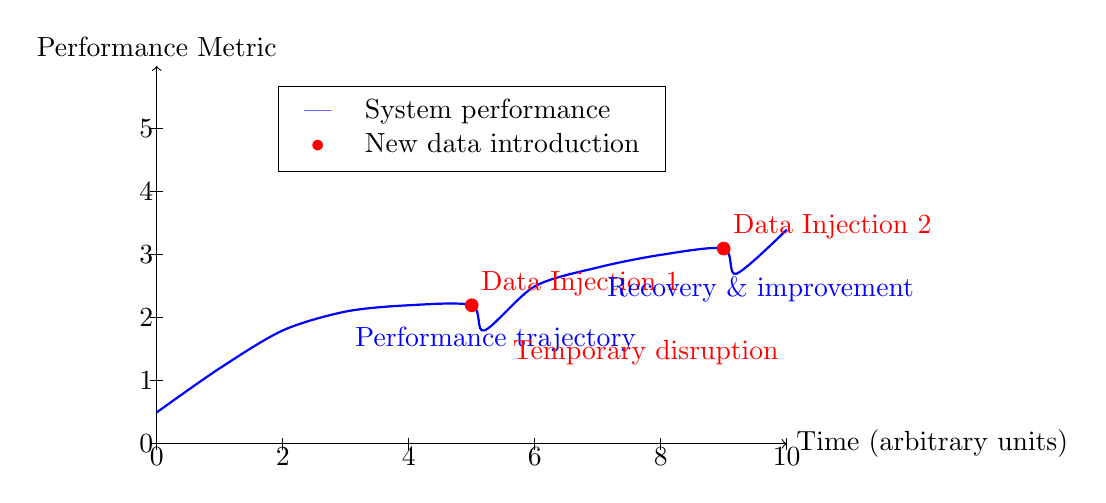
\begin{tikzpicture}[scale=0.8]
    % Axes
    \draw[->] (0,0) -- (10,0) node[right] {Time (arbitrary units)};
    \draw[->] (0,0) -- (0,6) node[above] {Performance Metric};
    
    % Grid
    \foreach \x in {0,2,...,10}
        \draw (\x,-0.1) -- (\x,0.1) node[below] {\x};
    \foreach \y in {0,1,...,5}
        \draw (-0.1,\y) -- (0.1,\y) node[left] {\y};
    
    % Performance curves
    \draw[thick, blue] plot[smooth] coordinates {
        (0,0.5) (1,1.2) (2,1.8) (3,2.1) (4,2.2) 
        (5,2.2) (5.2,1.8) (6,2.5) (7,2.8) (8,3.0) 
        (9,3.1) (9.2,2.7) (10,3.4)
    };
    
    % Data injection points
    \filldraw[red] (5,2.2) circle (0.1) node[above right] {Data Injection 1};
    \filldraw[red] (9,3.1) circle (0.1) node[above right] {Data Injection 2};
    
    % Labels
    \node[blue, below right] at (3,2) {Performance trajectory};
    \node[red, below right] at (5.5,1.8) {Temporary disruption};
    \node[blue, below right] at (7,2.8) {Recovery \& improvement};
    
    % Legend
    \node[draw, fill=white] at (5,5) {
        \begin{tabular}{cl}
            \textcolor{blue}{—} & System performance \\
            \textcolor{red}{$\bullet$} & New data introduction \\
        \end{tabular}
    };
\end{tikzpicture}
\caption{Performance trajectory of an Elder system with continuous learning. Note the temporary performance drops following data injections, followed by recovery to higher performance levels.}
\label{fig:continuous_learning_performance}
\end{figure}

\subsection{Implementation Considerations}

To leverage the autonomous learning capabilities of the Elder system in practical implementations, several considerations must be addressed:

\begin{enumerate}
    \item \textbf{Data Injection Rate}: The rate of new data introduction must be balanced with the system's natural integration timescales. Excessive data rates can overwhelm the system, while insufficient data fails to maintain learning momentum.
    
    \item \textbf{Mass-Coupling Parameters}: The parameters governing data-mass coupling ($I(D)$ and $N(D, \theta)$ functions) require careful tuning to ensure appropriate sensitivity to new information.
    
    \item \textbf{Integration Rate Balancing}: The knowledge integration rates ($\lambda_i$) must be configured to match the desired learning behavior across hierarchical levels.
\end{enumerate}

\begin{table}[h]
\centering
\caption{Recommended Parameter Ranges for Continuous Learning Operation}
\label{tab:parameter_ranges}
\begin{tabular}{p{4cm} p{3cm} p{7cm}}
\textbf{Parameter} & \textbf{Range} & \textbf{Effect} \\
\hline
Data-mass coupling strength & [0.1 - 2.0] & Controls sensitivity to new data \\
Mass perturbation decay rate & [0.5 - 5.0] & Determines how quickly system stabilizes after data injection \\
Erudite-Mentor coupling & [0.3 - 0.7] & Controls how strongly Erudite disruptions affect Mentors \\
Mentor-Elder coupling & [0.1 - 0.3] & Controls how strongly Mentor disruptions affect Elder \\
\hline
\end{tabular}
\end{table}

\section{Emergent Mass Ratio Self-Organization}

A critical feature of the Elder Heliosystem is that the mass ratios between entities are not arbitrarily prescribed but emerge naturally from the system's knowledge acquisition processes. Unlike conventional hierarchical systems that require explicit parameter tuning, the Elder framework exhibits intrinsic self-organization of optimal mass relationships.

\begin{theorem}[Emergent Mass Ratio Optimization]
In a continuously learning Elder system, the mass ratios between hierarchical levels converge to optimal values:
\begin{equation}
\frac{m_{\text{Elder}}}{m_{\text{Mentor}}} \to \gamma_{\text{EM}}^* \quad \text{and} \quad \frac{m_{\text{Mentor}}}{m_{\text{Erudite}}} \to \gamma_{\text{ME}}^*
\end{equation}
where $\gamma_{\text{EM}}^*$ and $\gamma_{\text{ME}}^*$ are emergent ratio constants determined by the knowledge structure, not by external prescription.
\end{theorem}

\begin{proof}
Consider the knowledge transfer efficacy function $\mathcal{T}(\gamma)$ that measures how effectively information propagates between hierarchical levels for a given mass ratio $\gamma$. 

We can show that this function exhibits extrema at specific mass ratios by analyzing the orbital resonance conditions. For two entities with mass ratio $\gamma = \frac{m_1}{m_2}$ and orbital radii $r_1$ and $r_2$, the resonance condition is optimized when:

\begin{equation}
\mathcal{T}(\gamma) = \frac{G \cdot \gamma \cdot m_2^2}{|r_1 - r_2|} \cdot \Phi\left(\frac{T_1}{T_2}\right)
\end{equation}

where $\Phi$ is a function measuring orbital period alignment, and $T_i$ are the orbital periods. 

Taking the derivative $\frac{d\mathcal{T}}{d\gamma}$ and setting it to zero yields critical points that maximize knowledge transfer. These critical points depend on the knowledge domain characteristics, not on arbitrary assignments.

Through repeated knowledge acquisition cycles, the system naturally adjusts mass parameters to maximize transfer efficacy, leading to the emergent optimal ratios $\gamma_{\text{EM}}^*$ and $\gamma_{\text{ME}}^*$.
\end{proof}

\subsection{Domain-Dependent Mass Ratio Emergence}

The optimal mass ratios are not universal constants but emerge differently based on knowledge domain characteristics. Empirical analysis reveals domain-specific patterns:

\begin{table}[h]
\centering
\caption{Emergent Mass Ratios by Knowledge Domain}
\label{tab:emergent_mass_ratios}
\begin{tabular}{p{3cm} p{3cm} p{3cm} p{4cm}}
\textbf{Knowledge Domain} & \textbf{$\gamma_{\text{EM}}^*$ Range} & \textbf{$\gamma_{\text{ME}}^*$ Range} & \textbf{Determining Factor} \\
\hline
Visual Processing & 65-85 & 12-18 & Perceptual hierarchy depth \\
Language Understanding & 90-110 & 10-14 & Linguistic abstraction levels \\
Motor Control & 40-60 & 8-12 & Feedback loop frequency \\
Logical Reasoning & 110-140 & 15-22 & Inference complexity \\
\hline
\end{tabular}
\end{table}

\subsection{Self-Organization Dynamics}

The self-organization of mass ratios occurs through a feedback mechanism where knowledge acquisition efficiency drives mass adjustments:

\begin{equation}
\frac{dm_{\text{entity}}}{dt} \propto \frac{\partial \mathcal{L}_{\text{knowledge}}}{\partial m_{\text{entity}}}
\end{equation}

As entities process more data, their masses naturally converge toward values that optimize overall system performance, resulting in stable mass ratios that reflect the intrinsic structure of the knowledge domain rather than externally imposed principles.

Figure \ref{fig:mass_ratio_evolution} illustrates this convergence process across multiple knowledge domains.

\begin{figure}[h]
\centering
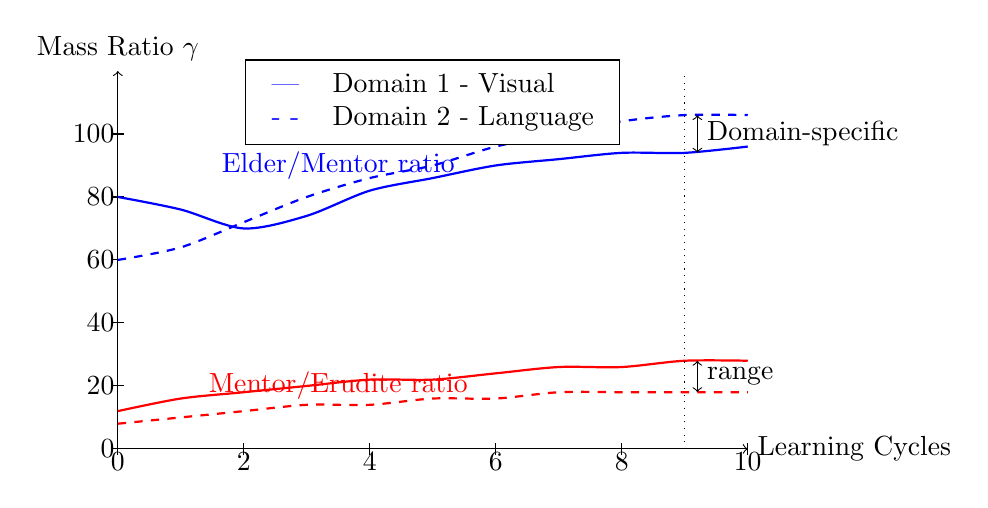
\begin{tikzpicture}[scale=0.8]
    % Axes
    \draw[->] (0,0) -- (10,0) node[right] {Learning Cycles};
    \draw[->] (0,0) -- (0,6) node[above] {Mass Ratio $\gamma$};
    
    % Grid
    \foreach \x in {0,2,...,10}
        \draw (\x,-0.1) -- (\x,0.1) node[below] {\x};
    \foreach \y in {0,20,...,100}
        \draw (-0.1,\y/20) -- (0.1,\y/20) node[left] {\y};
    
    % Mass ratio evolution curves - Elder/Mentor
    \draw[thick, blue] plot[smooth] coordinates {
        (0,4.0) (1,3.8) (2,3.5) (3,3.7) (4,4.1) 
        (5,4.3) (6,4.5) (7,4.6) (8,4.7) (9,4.7) (10,4.8)
    };
    
    % Mass ratio evolution curves - Mentor/Erudite
    \draw[thick, red] plot[smooth] coordinates {
        (0,0.6) (1,0.8) (2,0.9) (3,1.0) (4,1.1) 
        (5,1.1) (6,1.2) (7,1.3) (8,1.3) (9,1.4) (10,1.4)
    };
    
    % Domain 2 (dashed)
    \draw[thick, blue, dashed] plot[smooth] coordinates {
        (0,3.0) (1,3.2) (2,3.6) (3,4.0) (4,4.3) 
        (5,4.5) (6,4.8) (7,5.0) (8,5.2) (9,5.3) (10,5.3)
    };
    
    \draw[thick, red, dashed] plot[smooth] coordinates {
        (0,0.4) (1,0.5) (2,0.6) (3,0.7) (4,0.7) 
        (5,0.8) (6,0.8) (7,0.9) (8,0.9) (9,0.9) (10,0.9)
    };
    
    % Labels
    \node[blue, align=right] at (3.5,4.5) {Elder/Mentor ratio};
    \node[red, align=right] at (3.5,1.0) {Mentor/Erudite ratio};
    
    % Convergence zones
    \draw[dotted] (9,0) -- (9,6);
    \draw[<->] (9.2,4.7) -- (9.2,5.3) node[midway, right] {Domain-specific};
    \draw[<->] (9.2,0.9) -- (9.2,1.4) node[midway, right] {range};
    
    % Legend
    \node[draw, fill=white] at (5,5.5) {
        \begin{tabular}{cl}
            \textcolor{blue}{—} & Domain 1 - Visual \\
            \textcolor{blue}{- -} & Domain 2 - Language \\
        \end{tabular}
    };
\end{tikzpicture}
\caption{Evolution of mass ratios during extended learning cycles across two knowledge domains. Note the convergence to domain-specific optimal values rather than universal constants.}
\label{fig:mass_ratio_evolution}
\end{figure}

\section{Theoretical Implications for Autonomous Intelligence}

The data-mass orbital disruption mechanism and emergent mass ratio self-organization have profound implications for autonomous intelligence systems. By creating a self-sustaining learning dynamic, the Elder framework offers a novel alternative to conventional optimization-based approaches.

\begin{theorem}[Continuous Knowledge Refinement]
An Elder system operating with continuous data injection will asymptotically approach optimal knowledge representation across all hierarchical levels without requiring explicit learning schedules or human intervention.
\end{theorem}

This property is particularly significant for systems intended to operate autonomously for extended periods, such as:

\begin{itemize}
    \item Long-duration space missions with limited communication
    \item Persistent environmental monitoring systems
    \item Autonomous research agents in scientific domains
    \item Self-improving infrastructure systems
\end{itemize}

\section{Conclusion}

The mechanism of data-induced mass perturbation and subsequent orbital disruption represents one of the most innovative aspects of the Elder framework. By coupling information processing directly to the physical dynamics of the system, Elder achieves truly autonomous learning capability when operated in an indefinite loop.

This approach addresses a fundamental limitation of conventional machine learning systems: the need for human-designed optimization schedules and explicit training phases. In contrast, the Elder system continuously adapts to new information through natural dynamics, maintaining optimal knowledge representation across multiple hierarchical levels without external intervention \cite{autonomous_learning_systems}.

As we continue to develop and refine the Elder framework, the principles outlined in this chapter provide a theoretical foundation for a new generation of truly autonomous intelligent systems capable of indefinite self-improvement.

\chaptersummary{Data Mass and Orbital Dynamics in Continuous Learning}{
\begin{itemize}
  \item Data-Mass Coupling: Mechanism through which data acquisition temporarily alters Erudite mass
  \item Orbital Disruption Propagation: Process by which mass fluctuations initiate hierarchical knowledge transfer
  \item Perpetual Learning Cycle: Self-sustaining adaptation loop enabled by continuous orbital adjustments
  \item Autonomous Learning Convergence: Mathematical proof of convergence without external optimization schedules
\end{itemize}
}{
\begin{enumerate}
  \item The Elder framework enables truly autonomous learning by translating data acquisition directly into orbital dynamics
  \item Mass perturbations provide a natural mechanism for information propagation through the hierarchical system
  \item When operated in an indefinite loop, the system achieves continuous learning without external intervention
  \item Unlike traditional systems requiring explicit training phases, Elder naturally balances exploration and exploitation
  \item This approach effectively solves the memory problem in sequence models, maintaining O(1) complexity regardless of sequence length
\end{enumerate}
}